%%%%%%%%%%%%%%%%%%%% author.tex %%%%%%%%%%%%%%%%%%%%%%%%%%%%%%%%%%%
%
% template for chapters to the Handbook of Exoplanets
% modified by H. Deeg from the 'template.tex' provided by Springer for the svmult.cls class
% 20Mar 2016
%
%%%%%%%%%%%%%%%% Springer %%%%%%%%%%%%%%%%%%%%%%%%%%%%%%%%%%


% RECOMMENDED %%%%%%%%%%%%%%%%%%%%%%%%%%%%%%%%%%%%%%%%%%%%%%%%%%%
\documentclass[graybox,natbib,nosecnum]{svmult}
\bibpunct{(}{)}{;}{a}{}{,} % suppress commas between author-names and year

\pdfoutput=1   %forces use of pdflatex. Disable if you prefer to use .eps or .ps figures.
% choose options for [] as required from the list
% in the Reference Guide

\usepackage{mathptmx}       % selects Times Roman as basic font
\usepackage{helvet}         % selects Helvetica as sans-serif font
\usepackage{courier}        % selects Courier as typewriter font
\usepackage{type1cm}        % activate if the above 3 fonts are
                            % not available on your system

\usepackage{makeidx}         % allows index generation
\usepackage{graphicx}        % standard LaTeX graphics tool
                             % when including figure files
\usepackage{multicol}        % used for the two-column index
\usepackage[bottom]{footmisc}% places footnotes at page bottom
\usepackage[normalem]{ulem}	% for strike-through of text with \sout{}  
\usepackage{hyperref}  %for hyperlinks

\usepackage{soul}   % for high-lighting of text
% see the list of further useful packages
% in the Reference Guide

% expansions of  journal abbreviations from bibtex entries by ADS
% adapted to Springer Basic style (no periods in abbreviations)
\newcommand*\aap{A\&A}
\let\astap=\aap
\newcommand*\aapr{A\&A Rev}
\newcommand*\aaps{A\&AS}
\newcommand*\actaa{Acta Astron}
\newcommand*\aj{AJ}
\newcommand*\ao{Appl Opt}
\let\applopt\ao
\newcommand*\apj{ApJ}
\newcommand*\apjl{ApJ}
\let\apjlett\apjl
\newcommand*\apjs{ApJS}
\let\apjsupp\apjs
\newcommand*\aplett{Astrophys Lett}
\newcommand*\apspr{Astrophys Space Phys Res}
\newcommand*\apss{Ap\&SS}
\newcommand*\araa{ARA\&A}
\newcommand*\azh{AZh}
\newcommand*\baas{BAAS}
\newcommand*\bac{Bull astr Inst Czechosl}
\newcommand*\bain{Bull Astron Inst Netherlands}
\newcommand*\caa{Chinese Astron Astrophys}
\newcommand*\cjaa{Chinese J Astron Astrophys}
\newcommand*\fcp{Fund Cosmic Phys}
\newcommand*\gca{Geochim Cosmochim Acta}
\newcommand*\grl{Geophys Res Lett}
\newcommand*\iaucirc{IAU Circ}
\newcommand*\icarus{Icarus}
\newcommand*\jcap{J Cosmology Astropart Phys}
\newcommand*\jcp{J Chem Phys}
\newcommand*\jgr{J Geophys Res}
\newcommand*\jqsrt{J Quant Spectr Rad Transf}
\newcommand*\jrasc{JRASC}
\newcommand*\memras{MmRAS}
\newcommand*\memsai{Mem Soc Astron Italiana}
\newcommand*\mnras{MNRAS}
\newcommand*\na{New A}
\newcommand*\nar{New A Rev}
\newcommand*\nat{Nature}
\newcommand*\nphysa{Nucl Phys A}
\newcommand*\pasa{PASA}
\newcommand*\pasj{PASJ}
\newcommand*\pasp{PASP}
\newcommand*\physrep{Phys Rep}
\newcommand*\physscr{Phys Scr}
\newcommand*\planss{Planet Space Sci}
\newcommand*\pra{Phys Rev A}
\newcommand*\prb{Phys Rev B}
\newcommand*\prc{Phys Rev C}
\newcommand*\prd{Phys Rev D}
\newcommand*\pre{Phys Rev E}
\newcommand*\prl{Phys Rev Lett}
\newcommand*\procspie{Proc SPIE}
\newcommand*\qjras{QJRAS}
\newcommand*\rmxaa{Rev Mexicana Astron Astrofis}
\newcommand*\skytel{S\&T}
\newcommand*\solphys{Sol Phys}
\newcommand*\sovast{Soviet Ast}
\newcommand*\ssr{Space Sci Rev}
\newcommand*\zap{ZAp}


\newcommand{\hbindex}[1]{\hl{#1}\index{#1}}  %highlights index entries

\makeindex             % used for the subject index
                       % please use the style svind.ist with
                       % your makeindex program

%%%%%%%%%%%%%%%%%%%%%%%%%%%%%%%%%%%%%%%%%%%%%%%%%%%%%%%%%%%%%%%%%%%%%%%%%%%%%%%%%%%%%%%%%

\begin{document}

\title*{Title: Transit Timing and Duration Variations for the Discovery and Characterization of Exoplanets}
% Use \titlerunning{Short Title} for an abbreviated version of
% your contribution title if the original one is too long
\author{Eric Agol and Daniel C.\ Fabrycky}
% Use 
\authorrunning{Transit timing} % for an abbreviated version of
% your contribution title if the original one is too long
\institute{Eric Agol \at Department of Astronomy, Box 351580, University of Washington, Seattle, WA 98195-1580, USA \email{agol@uw.edu}
\and Daniel C.\ Fabrycky \at Dept.\ of Astronomy \& Astrophysics, University of Chicago, Chicago, IL 60637, USA \email{fabrycky@uchicago.edu}}
%
% Use the package "url.sty" to avoid
% problems with special characters
% used in your e-mail or web address
%
\maketitle


\abstract{Transiting exoplanets in multi-planet systems have non-Keplerian orbits which can cause the times and durations of transits to vary.  We review the theory and observations of transit timing variations (TTV) and transit duration variations (TDV).}

\section{Introduction}

Here we discuss some aspects of planetary orbital physics, to set the stage for TTV and TDV.  Consider the vector stretching from the star of mass $M_\star$ to the planet of mass $M_p$ to be $\mathbf{r}=(x,y,z)$, with a distance $r$ and direction $\mathbf{\hat r}$.  The Keplerian potential, $\phi=-GM/r$ (where $M \equiv M_\star + M_p$ and the planet is replaced with a body of reduced mass $\mu \equiv M_\star M_p / (M_\star+M_p)$), is one of only two radial, power-law potentials that gives rise to closed orbits \footnote{the other one, the harmonic potential $-kr$ would only have relevance for collisionless orbits within a homogeneous massive body}.  This means that, in the absense of perturbations, there is a strict periodicity $\mathbf{r}(t+P) = \mathbf{r}(t)$.  Moreover, Kepler showed that Tycho Brahe's excellent data for planetary positions were consistent with Copernicus' idea of a heliocentric system only if the planets (including the Earth) followed elliptical paths of semi-major axis $a$, and one focus on the Sun. Newton was successful at finding the principle underlying such orbits, a force law $\mathbf{F} = \mu \mathbf{\ddot r} =-G \mu M r^{-2} \mathbf{\hat r}$, which results in a period $P = 2 \pi a^{3/2} G^{-1/2} (M_\star + M_p)^{-1/2}$ (i.e. with the $a$-scaling Kepler found the planets actually obeyed).

This research program was thrown into some doubt by the ``Great Inequality,'' the fact that the orbits of Jupiter and Saturn did not fit the fixed Keplerian ellipse model.  This was overcome by the perturbation theory of Laplace, who used the masses derived via their satellite orbits to explain their deviations of their solar orbits \citep{1985Wilson}.  We can recreate the main effect of this insight by writing an additional force to that of gravity of the Sun: 
\begin{equation}
\mathbf{F_{1}} = -G \mu_1 M r_{1}^{-2} \mathbf{\hat r_{1}} + \mathbf{F_{21}},
\end{equation}
where we now specify forces and distances explicitly to planet 1, and add a force of planet 2 on planet 1.  This latter force consists of two terms: 
\begin{equation}
\mathbf{F_{21}} = \mu_1 \mathbf{\ddot r_1} = -G \mu_1 M_2 \vert r_{1}-r_{2}\vert^{-3} (\mathbf{r_{2}} - \mathbf{r_{1}}) + G \mu_1 M_2 r_{2}^{-2} \mathbf{\hat r_{2}}.
\end{equation}
The first term on the right-hand-side is the direct gravitational acceleration of planet 1 due to planet 2.  The second is a frame-acceleration effect, due to the acceleration the Sun feels due to the second planet.  Since the Sun is fixed at the zero of the frame, this acceleration is manifested by acceleration in the opposite direction of planet 1.  

Likewise, Leverrier and Adams used the same technique, dynamical perturbations, to discover the first planet by gravitational means \citep{Adams1847,LeVerrier1877}. In this case, they did not know the zeroth order solution (i.e. the Keplerian ellipse) for the yet-to-be-discovered Neptune.  In its place, they assumed the Titius-Bode rule held, and sought only the phase of the orbit.  This worked because they only wanted to see how the acceleration, then deceleration, as Uranus passed Neptune, would betray its position on the sky to optical observers.  [Say later: the task that researchers set for themselves to discover planets by TTV is a bit more demanding.  We do not have any hints as to what the planet's orbit might be (neither circular nor roughly obeying some spacing law).  Additionally, the data per orbit is considerably noisy; in only a few cases are the orbit-by-orbit ``chopping'' signal statistically significant after just three transits. Finally, the orbit is only sampled at the transit phase, so opportunities for aliasing of the signal are abundant.]

The discovery of transits marks the first time that data on exoplanets could be precise enough to notice gravitational interactions.\footnote{Only around the same time (2000) were perturbations noticed in the resonant interaction of the planets of GJ 876 \citep{2001Laughlin}.}  The times of transit are primarily constrained by the decline of stellar flux during transit ingress, and the rise over egress, which occur on a timescale 
\begin{equation} \label{ingress}
\tau \approx \pi^{-1} P(R_p/a) \approx 10^{-4}P \left(\frac{3 R_p}{R_\oplus}\right) \left(\frac{a}{0.3 \rm{AU}}\right)^{-1},
\end{equation}  
assuming an impact parameter of $b=0$.
This allows the transit times to be measured precisely relative to the orbital period, giving a sensitive measure of the variation of the angular position of a planet relative to a Keplerian orbit.  In contrast, the stellar radial velocity varies on the orbital timescale, and thus the precision of the orbital phase is poorly constrained unless the measurements are of high precision or long duration (which allows deviations to grow with time).

We may define express the orbital positions or transit times in a table called an ephemeris, and the perturbations would be the motions or timing deviations that go beyond a Keplerian reference model.  In the case of transit timing variations, the Keplerian alternative is simply an ephemeris with a constant transit period, $P$:
\begin{equation}
C = T_0 + P \times E, 
\end{equation}
where $E$ is the integer number of a transit and $T_0$ is the time of the first transit; $C$ stands for ``calculated'' based on a constant-period model.  Meanwhile, the Observed times of transit are denoted $O$.  This notation leads to an ``O minus C'' diagram, in which only the perturbation part is plotted.  An instructive version, modelled after the timing of WASP-47 \citep{2015Becker} but with a greatly exaggerated perturbation, is shown in figure~\ref{omc}. 
\begin{itemize}
\item Definition of TTVs/TDVs [DF] (Figure? O-C method)
     \citep{2005Sci...307.1288H,2010Sci...330...51H}
%\item History: theory, observation  (Schneider TTV, Miralda-Escude' TTV) [EA] \citep{2002ApJ...564.1019M,2010Sci...330...51H}
\end{itemize}

% For figures use
\begin{figure}
\centerline{
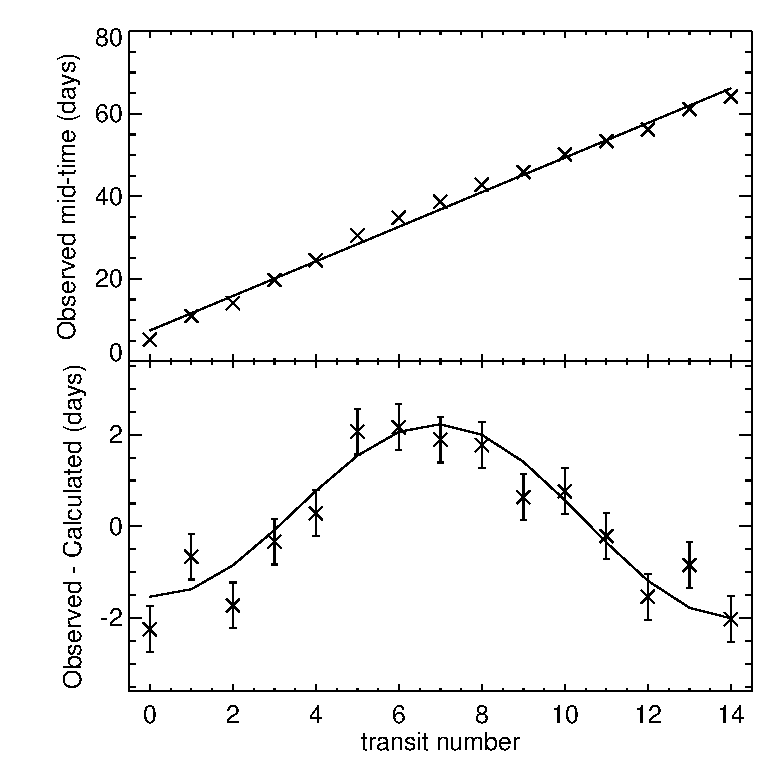
\includegraphics[width=0.9\textwidth]{omc.eps}}
%
\caption{An example of timing data.  {\emph Top panel}: the measured midtimes of exoplanet transits, to which a line is fit by least-squares.  {\emph Bottom panel}: the residuals of that fit, which is the conventional $O-C$ diagram; the original sinusoidal function, to which Gaussian noise was added, is also plotted as a line. }
\label{omc}       % Give a unique label
\end{figure}


The literature on exoplanets has a history of rediscovering effects that had been well studied in the field of binary stars.  Radial velocity, transits/eclipses, the Rossiter-McLaughlin effect, astrometry, and high-contrast imaging have all been used in the study of multi-star sytems.  Stars, however, are only stable in a hierarchical configuration so that only secular or tidal dynamics can play a role in triple star systems \citep{2003A&A...398.1091B}.  Planetary systems can be much more compact due to the dominant mass of the central star, and so mean-motion resonances can dominate the dynamics of multi-planet systems.  Transit-timing variations due to mean-motion resonances is a novel aspect of exoplanet systems that did not play a role in the study of multi-star systems.  

The first recognition of the importance of transit timing and duration variations was at the DPS and AAS meetings two decades ago by \citet{1996DPS....28.1208D,1996BAAS...28.1112D}, followed a few years later by \citet{2002ApJ...564.1019M} and \citet{Schneider2003,Schneider2004}.  More detailed studies which included the important effect of mean-motion resonance were submitted simultaneously by \citet{2005Sci...307.1288H} and \citet{2005MNRAS.359..567A}.  The former paper showed that Solar-system like perturbations might be used to find Earth-like planets, should transit times be measured with sufficient accuracy.  The latter paper coined the term `transit-timing variations,' with acronym TTVs, and defined TTVs as being the residuals of a linear fit to the times of a transiting planet.

Initial studies of TTVs of hot Jupiters were able to place limits on the presence of Earth-mass planets near mean-motion resonance.  Some further studies claimed detection of perturbing planets causing TTVs or TDVs, but each of these were quickly disputed or refuted by additional measurements.  The first convincing detection awaited the launch of the Kepler spacecraft, and the detection of Kepler-9 which showed large-amplitude TTVs of two Saturn-sized planets with strong significance \citep{2010Sci...330...51H}; this discovery was remarkably similar to predictions that had been made based upon the GJ 876 system \citep{2005MNRAS.359..567A}.  This paper kicked off a series of discoveries of TTVs with the Kepler spacecraft, with now more than 100 systems displaying TTVs, and a handful showing TDVs.

% Ribas (2008) 2008ApJ...677L..59R claimed a detection from TDV, but ruled out by Alonso et al. (2008) 2008A&A...487L...5A
% Ribas (2009) defended his case 2009IAUS..253..149R
% Diaz claimed TTVs of OGLE-TR-111b 2008ApJ...682L..49D; Adams et al. (2010) ruled it out 2010ApJ...714...13A
% Maciejewski et al. (2010) claimed TTV of WASP-3b, which was refuted by Montalto (2012) 2012MNRAS.427.2757M, 
%  Nascimbeni (2013) 2013A&A...549A..30N & Maciejewski (2013) 2013AJ....146..147M.  
% WASP-3b TDV claim was made by Eibe et al. (2012) 2012MNRAS.423.1381E

\section{Preliminaries}

Since the gravitational interactions between planets occurs on the orbital timescale, the
amplitude of transit timing variations is proportional to the orbital period of each planet,
as well as a function of other dimensionless quantities.  Thanks to Newton's second law
and Newton's law of gravity, the acceleration of a body does not depend on its own mass.
Thus, the transit timing variations of each planet scale with the masses of the {\it other} bodies
in the system.
In a two-planet system, then, to lowest order in mass ratio,
\begin{eqnarray}
\vert \delta t_1\vert &=& \frac{P_1}{2\pi} \frac{m_2}{m_0} f_{12}(\alpha_{12},\mathbf{x}_{12}),\cr
\vert \delta t_2\vert &=& \frac{P_2}{2\pi} \frac{m_1}{m_0} f_{21}(\alpha_{12},\mathbf{x}_{21}),
\end{eqnarray}
where the masses of the star and planets are $m_0, m_1,$ and $m_2$, and $f_{ij}$ governs
the timing variations of planet $j$ on planet $i$,
which is a function of the semi-major axis ratio, $\alpha_{12}= a_1/a_2 < 1$, and the angular orbital 
elements of the planets, $\mathbf{x}_{ij} = (\lambda_i,\omega_i,I_i,\Omega_i,\lambda_j,\omega_j,I_j,\Omega_j)$.

%  - Basic scalings: $\propto$P, $\propto m/M_{star}$ for the perturber, stronger near resonance [EA]
\begin{itemize}
\item Energy/angular momentum conservation [DF]
\end{itemize}

%  - Linear TTV (independently adds from different planets, off resonance)  - 
With the addition of multiple perturbing planets, if the mass-ratios of the planets to the star is
sufficiently small and if none of the planets exist in a resonant configuration, then the transiting timing 
variations may be approximately expressed as linear combinations of the perturbations due to each companion.
For $N$ planets, the TTVs become
\begin{equation}
\delta t_j = P_j \sum_{i \ne j}  \frac{m_i}{m_0} f_{ij}(\alpha_{ij},\mathbf{x}_{ij}).
\end{equation}
Note that $\alpha_{ij} = {\rm min}(a_i/a_j,a_j/a_i)$.

The measurement of TTVs and TDVs has been used for confirmation, detection, and characterization of
transiting exoplanets and their companions.  The Kepler spacecraft discovered thousands of transiting
exoplanet candidates;  the classification as `candidate' was cautiously used to allow for other
possible explanations, such as a blend of a foreground star and a background eclipsing binary causing
an apparent transit-like signal.  The presence of multiple transiting planets around the same star
gave a means of confirming two planets that display {\em anti-correlated} TTVs: due to energy and
angular momentum conservation, the anti-correlation indicates dynamical interactions between the
two planets, while such a configuration would not be stable for a triple star system.  A series of papers 
used this technique to confirm that Kepler planet candidates were bonafide exoplanets:
\citet{2011ApJS..197....2F, 2012ApJ...750..113F, 2012ApJ...750..114F, 2012ApJ...756..185F, 
2012MNRAS.421.2342S, 2013MNRAS.428.1077S, 2013ApJS..208...22X, 2014ApJS..210...25X}.

The confident detection of perturbing exoplanets with TTVs awaited the Kepler spacecraft as
well.  The Kepler-19b planet showed sinusoidal TTVs that were used to identify a handful
of possible planet period and mass combinations that might be responsible for the perturbations \citep{2011ApJ...743..200B}.
The unique identification of a perturbing planet was accomplished with Kepler-46 (aka KOI-872)
which displayed very high signal-to-noise TTVs which allowed the period and mass of the
perturber to be measured with some precision \citep{2012Sci...336.1133N}.  The detection
and characterization of a perturbing planet in KOI-142 required both TTV and TDV \citep{2013ApJ...777....3N}.

The characterization of exoplanets with TTVs also began in earnest with the Kepler spacecraft.
In addition to Kepler-9, the Kepler-18 system was characterized by a combination of TTVs and
RVs, giving density estimates for the three transiting planets \citep{2011ApJS..197....7C}.

The characterization of exoplanets is complicated by degeneracy between mass and eccentricity
caused by aliasing at the frequency of the transiting planet (discussed below).  However,
in general transit timing variations gives a means of measuring the density of exoplanets.
The two observables associated with a light curve are the time stamp of each photometric
measurement and the number of photons measured.  The number of photons is a dimensionless
number, and thus may only constrain dimensionless quantities, such as radius ratio, impact 
parameter, or the ratio of the stellar size to the semi-major axis.  The quantities that 
have units of time --- the period, transit duration, ingress duration ---  can further
constrain the density of the system since the dynamical time $t_{dyn} \approx
(G\rho)^{-1/2}$.  \citet{2003ApJ...585.1038S} showed that a single transiting planet
on a well-measured circular orbit may be used to gauge the density of the star;
in the case of multiple transiting planets, the circular assumption may be relaxed
\citep{2014MNRAS.440.2164K}.
The transit depth, then, gives the radius-ratio of the planet to the star, while if two
transit and show TTVs, their TTVs give an estimate of the mass ratio of their perturber
to the star.  Thus, two transiting, interacting planets yield an estimate of the density ratio of
the planets to the star, and consequently we can obtain the density of the planets.
Note that this is true even if the absolute mass and radius of the star are poorly
constrained.  A caveat to this technique is that there is an eccentricity dependence that 
is present in TTVs as well,
but typically multi-transiting planet systems require low eccentricities to be stable,
and in some cases the eccentricities can be constrained sufficiently from TTVs, from
analyzing multiple planets \citep{2014MNRAS.440.2164K}, or
statistically from an ensemble analysis \citep{2014ApJ...787...80H}, so this ends up not impacting the stellar density 
estimate significantly, although it can impact the planet-star mass ratios, and
hence inflate the planet density uncertainty.
Another way to obtain an estimate of stellar density is from asteroseismology:
in fact, the time dependence of asteroseismic measurements is what enables density
to be constrained in that case as well \citep{1986ApJ...306L..37U}.

If a pair of transiting exoplanets can be detected with {\it both} TTVs and RVs, then the
absolute dimensions of the system can be obtained \citep{2005MNRAS.359..567A,
2013ApJ...762..112M} as RVs have a dimensions of velocity, which 
when combined with time measurements from TTVs gives dimensions of distance.
In practice this technique has yet to yield useful constraints upon the properties
of planetary systems \citep{2015MNRAS.453.2644A}, but it may prove fruitful
in the future much as double-lined spectroscopic binaries have used to measuring 
the properties of binary stars.  Circumbinary planets are an extreme example
of this technique: the timing offsets of the transits, combined with the eclipses
and radial-velocity of the binary give very precise constraints on the absolute parameters
of the Kepler-16 system \citep{2011Sci...333.1602D}.

%  - Applications: [EA]
%    - Detection
%    - Confirmation
%    - Characterization
%      - Sensitive to density since time-dependent: transits are sensitive to density of star; 
%   TTV are sensitive to mass ratio; transit depth radius ratio - so we get density of 
%   planet from transits + TTV.   Dimensions of G are density and time.
%      - TTV + RV gives Mass + radius ;   CBPs as example  

\section{Theory} % (applied to specific systems - show fits to actual data - either N-body or analytic)
  - TTVs:
    - Inner Keplerian variation;  CBPs as example (Kepler-16) [DF]
    - Near-resonant TTVs - Lithwick et al. \citep{2012ApJ...761..122L} [DF] (Figure - mechanism + data)
       - Degeneracy - multiple resonances can give same solution (Kepler-19); Breaking degeneracy with TDV as well [DF]
%    - Chopping/other harmonics - KOI 1353 / KOI-872 [EA] (Figure)
\subsection{Chopping}

When two planets are nearly resonant, the degeneracy between the mass ratios of the planets to the star
and the eccentricity vector may be broken by examining additional non-resonant harmonics present in the data \citep{2015ApJ...802..116D}.
These additional harmonics have a smaller amplitude due to the fact that they are not caused by resonant terms,
and thus require higher signal-to-noise to break the degeneracy between the mass and eccentricity.
Nevertheless, the chopping component can be detected in many cases, and leads to a unique measurement
of the masses of the exoplanets \citep{2014ApJ...790...58N,2014ApJ...795..167S,2015ApJ...802..116D}.

As an example, consider a pair of planets with period ratio of $P_2/P_1 = 1.52$.  This period ratio
is close to 3:2, and thus is affected by this resonant term, giving a TTV period of $75 P_1$.
Figure \ref{ttv_chopping} compares two planets with this period ratio with zero eccentricity
and mass-ratios of $10^{-6}$ to a pair of planets with eccentricites of $e_1=e_2=0.04$
and mass-ratios near $10^{-7}$.  Both pairs of planets give nearly identical amplitudes
for the resonant term, while the larger mass ratio planets show a much stronger chopping
variation.  In this case there is a clear difference between the TTVs of the two simulated
systems:  the inner planet shows a drift over three orbital periods, and a sudden jump
every third orbital period, while the outer one shows a similar pattern over two orbital
periods.  These variations are due to perturbations at integer multiples of the synodic
frequency, which has a period $P_{syn}^{-1} = 1/P_1-1/P_2$.  In this example we have
set the phase of the orbital parameters to be such that the TTVs match;  change
in the phase can also be indicative of a non-zero eccentricity contributing to the TTVs,
and with an ensemble of planets which are believed to have a similar eccentricity
distribution, the mass-eccentricity degeneracy may be broken statistically \citep{2012ApJ...761..122L,
2014ApJ...787...80H}.

% For figures use
\begin{figure}
\centerline{
\includegraphics[width=0.9\textwidth]{ttv_chopping.png}}
%
\caption{Transit-timing variations of two low-eccentricity planets with larger
mass ratios, $m_1 = m_2 = 10^{-6} m_*$ (green) compared with two higher eccentricity planets ($e_1=e_2=0.04$)
with smaller mass ratios $m_1 = m_2 = 10^{-7} m_*$.  The zig-zag chopping component
is apparent in the high-mass/low-eccentricity case, while less apparent in the low-mass/
high-eccentricity case.}
\label{ttv_chopping}       % Give a unique label
\end{figure}


    - Resonance - Kepler-30?  Ne'svorny (1603.07306); Boue'+2012 - Kepler-223 (resonant chain - to fit data \& stability); room for more work on this.  [DF]
    - Exomoons [EA]
    - Light time?  Borkovits deconvolution [DF]
    - Borkovits(?) - KOI 1474 {cleaner example?  Or leave out?  Future -- circumstellar planets in binaries; Schwartz et al. w/ Haghighipour.} [DF]     - TDVs
       - Precession - Kepler-108 {1606.04485} / KOI-142 {Nesvorny} / KOI-13 (Mazeh) - and CBPs turning on or off.  [DF]  Ragozzine/Wolf/Pal/Koscis/Jordan - GR precession - Heyl \& Gladman; J2  (Figure - CBP? - Kepler-47? Kostov? Kepler-35? Try them out.)

\section{Observations/Practical considerations} % [EA]
Confirmation of multi-planet systems in Kepler anti-correlated sinusoids, Ford GPs [DF]
%  [ Some firsts to history section; some best-cases as examples in theory section ]
%  - Timing precision: [EA]

\subsection{Timing precision}

The steepest portions of a transit are the ingress and egress when the planet crosses onto and
off of the disk of the star, causing a dip of depth $\delta = (R_p/R_*)^2$ if we ignore limb-darkening.   
Suppose for the moment that the only source of noise is Poisson noise due to the count rate of 
the star, $\dot N$.  The photometric precision over the duration of ingress scales as
$(\dot N \tau)^{1/2}$, where $\tau$ is the ingress duration (eqn.\ \ref{ingress}).  If the time of 
ingress fit from a model is offset by $\sigma_g$, then the difference in counts observed
versus the model is $\sigma_g \delta \dot N$ (the pink region in Fig.\ \ref{fig:ingress}).  Equating 
this to photometric uncertainty gives $\sigma_g = \tau^{1/2} \dot N^{-1/2} \delta^{-1}$, which
is the 68.3\% confidence timing precision assuming that the exposure time is much shorter than the
ingress duration and that $\sigma_g \ll \tau$.  The same formula applies to egress. A longer transit 
ingress duration leads to a shallower slope in ingress, which makes it more difficult to measure an 
offset in time of the model.  Higher count rates and deeper transits improve the precision, as 
expected.  Note that we've assumed that the duration of the transit is sufficiently long that the 
error on $\delta$ is small.

Suppose the transit duration is $T$.  Then, the uncertainty on the duration is given by
the sum of the uncertainties on the ingress and egress, added in quadrature:
$\sigma_T = \sqrt{2} \sigma_g$.  The timing precision, $\sigma_t$, is set by the mean of the ingress
and egress, giving $\sigma_t = \frac{1}{\sqrt{2}} \sigma_g$.

A more complete derivation of these expressions is given by \citet{2008ApJ...689..499C}, while an 
expression which includes the effects of a finite integration time is given by \citet{2014ApJ...794...92P}.
The assumptions of no limb-darkening and Poisson noise are generally broken by stars;  in addition,
stellar variability contributes to timing uncertainty, for which there is yet to be a general
expression.  These effects generally increase the uncertainty on the measurement of transit times
and durations, and so the best practice would be to estimate the timing uncertainties from the
data, accounting for effects of correlated stellar variability by including the full covariance
matrix of the timing uncertainty \citep{2009ApJ...704...51C,2012MNRAS.419.2683G}.  Crossing of
the path of the planet across star spots may also cause some uncertainty on the timing precision;
this can be diagnosed by a larger scatter within transit than outside transit or other signs of
significant stellar activity, and can be handled best by including the spots in the transit model 
\cite{2016A&A...585A..72I}.

% For figures use
\begin{figure}
% Use the relevant command for your figure-insertion program
% to insert the figure file.
% For example, with the graphicx style use
\centerline{
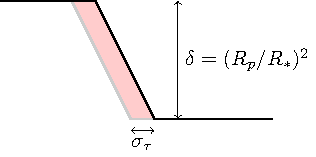
\includegraphics[width=0.5\textwidth]{ingress.pdf}}
%
\caption{Diagram of the transit ingress of a planet.  The precision of the timing of ingress, $\sigma_g$, is set by
when the area of the ingress (pink) equals the timing precision over the duration of ingress.}
\label{fig:ingress}       % Give a unique label
\end{figure}

%     - Comes from steepest part of lightcurve ingress/egress
%     - Signal-to-noise of TTV/TDV measurements (Carter/Winn; Rogers/Page)
%     - Finite-exposure time effects
%     - Effects of stellar variability: flux variability, star spots.

\section{Science Results}

The best characterized pair of planets to date using TTV reside in the Kepler-36 system \citep{2012Sci...337..556C}.  As this planet pair is close to a 6:7 period ratio, the conjunctions cause a significant kick to each planet resulting a TTV amplitude that is $\approx 1$\% of the orbital periods of the planets.  Figure \ref{fig:kep36} shows a `river-plot' for all seventeen quarters of long-cadence Kepler data for this pair of planets.  After each 7(6) orbits of the inner(outer) planet, there is a conjunction which causes a change in the eccentricity vector and period of each planet.  The change in the eccentricity vector causes a sudden change in the subsequent transit time, while the change in period causes a change in slope;  these are apparent for Kepler-36c in Figure \ref{fig:kep36}.  The large TTVs enable a precise measurement of the planet-star mass ratios for both planets (using the TTVs of the companion planet), while the star shows asteroseismic variability which gives precise planets for the stellar mass.   The net result are masses with uncertainties of $<8$\%, which is precise for planets of this size.  The inner planet shows a density which is consistent with scaling up the composition of Earth, while the outer planet requires a significant H/He envelope to explain its size which is comparable to Neptune \citep{2012Sci...337..556C}.

\begin{figure}
\centerline{
\includegraphics[width=0.9\textwidth]{Kepler36/Kepler36_river.png}}
\caption{River plot of Kepler-36b (left) and Kepler-36c (right).}
\label{fig:kep36}
\end{figure}


%    - Best characterization, specifically mass: Kepler-36 - conjunctions/impulse/Hill approximation (N-body) [EA]\\
    - Other favorite systems? Kepler-11 puffy/packed planets  [DF]\\
    - Best eccentricity constraint for a super-Earth?  Kepler-36? Include? \\
    - Ensemble TTV analysis: Xie - differing architecture for the single-transiters due to less frequent TTV, Hadden-Lithwick - eccentricity distribution; Hot Jupiters lonely (Steffen); Latham     - gas giants less frequent in multi-transiting (no TTVs)  [DF]\\
    - Measuring masses - Steffen bias?    [DF]\\
%    - N-body modeling of Kepler-systems: Jontof-Hutter  [DF] (Mass-radius Figure? - ask Daniel Jontof-Hutter)  Transparency to avoid big error bars visually dominating.  EA will make the figure.  Referenced Wayne Hu figure on cosmo constraints.\\
    - CBPs   [DF]

Catalogs of transit times have been produced for the multi-planet Kepler systems \citep{2013ApJS..208...16M,2016ApJS..225....9H}. Several analyses of an ensemble of TTV pairs of planets have recently been carried out \citep{{2014ApJ...787...80H,2013ApJS..208...22X,2014ApJS..210...25X,2016ApJ...820...39J}, with the largest by Hadden \& Lithwick (2016).  With a slightly smaller sample, we have selected only planets with mass precisions of better than $3-\sigma$ in Figure \ref{fig:density_period}.  There appears to be a trend of mean density decreasing with orbital period (one exception is K2-3d, although the authors warn its RV mass may be affected by stellar variability).  At periods near $\approx 10$ days, the RV and TTV densities agree rather well.  At shorter period, most of the RV detections are single-planets, whic in general appear to have lower density relative to their multi-planet counterparts.  When radius is plotted versus mass, and color-coded as a function of flux, Fig.\ \ref{fig:density_period}, there is a general trend radius increasing with mass, albeit with a large scatter in mass, while a handful of of `puffy' planets (with masses measured with TTV) show absurdly large radii given their small masses.  These mass measurements are surprising, but difficult to dispute as larger masses would have led to a larger, and hence easier-to-measure, TTV signal.

\begin{figure}
\centerline{
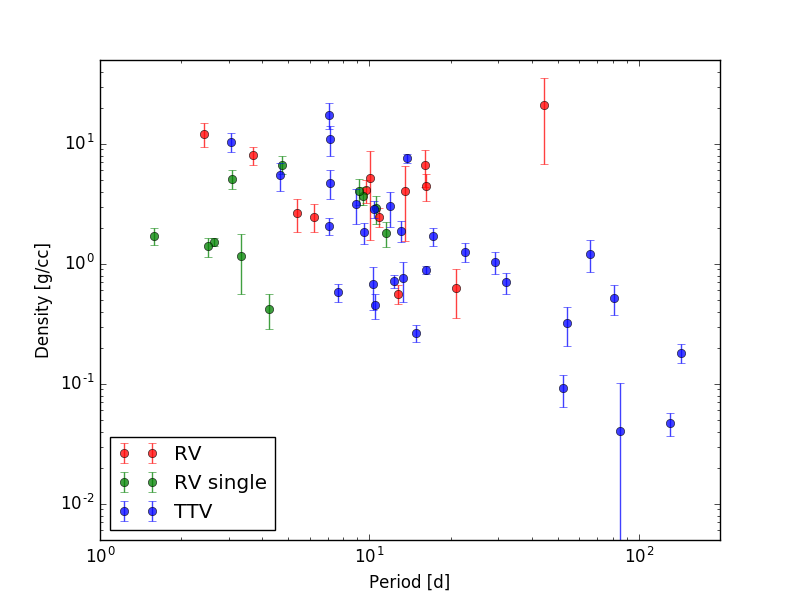
\includegraphics[width=0.95\textwidth]{density_vs_period_errors.png}}
\centerline{
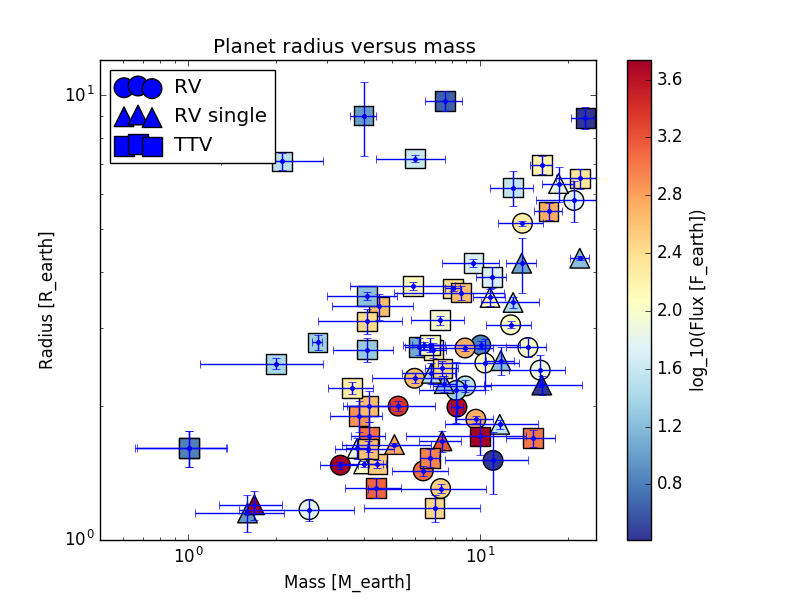
\includegraphics[width=0.95\textwidth]{mass_radius_flux.png}}
\caption{Density vs.\ period for planets transiting planets with masses $<25 M_\oplus$ (left).  Radius
vs.\ mass, with color indicating incident stellar flux (right).}
\label{fig:density_period}
\end{figure}


\section{Future} %  [Might have to chop, or at least briefly cover.  Assign at that time!]
  - More thorough TTV analysis: GPs - for measuring transit times
  - Follow-up of Kepler targets
  - Comparison of TTV masses with RV masses:  better constraints
    and confidence in both methods?
  - MCMC with high-multiplicity systems
  - TESS, JWST, CHEOPS, PLATO, ?
  - TTV/TDV of exomoons
  - HZ exoplanets
  - Smaller CBPs
  - Stellar/planet characterization: TTV + RV

References:

Borucki \& Summers
Struve
Cabrera
Charbonneau 2000

Neptune:
Bouvard/Adams/Le Verrier/Galle

%% For figures use
%\begin{figure}
%% Use the relevant command for your figure-insertion program
%% to insert the figure file.
%% For example, with the graphicx style use
%\includegraphics[scale=.65]{template_fig1}
%%
%\caption{Example figure. You do not have to worry on the layout as this will be revised by Springer}
%\label{fig:1}       % Give a unique label
%\end{figure}

%\begin{table}
%\caption{Please write your table caption here.}
%\label{tab:1}       % Give a unique label
%%
%% Follow this input for your own table layout
%%
%\begin{tabular}{p{2cm}p{2.4cm}p{2cm}p{4.9cm}}
%\hline\noalign{\smallskip}
%Classes & Subclass & Length & Action Mechanism  \\
%\noalign{\smallskip}\svhline\noalign{\smallskip}
%Translation & mRNA$^a$  & 22 (19--25) & Translation repression, mRNA cleavage\\
%Translation & mRNA cleavage & 21 & mRNA cleavage\\
%Translation & mRNA  & 21--22 & mRNA cleavage\\
%Translation & mRNA  & 24--26 & Histone and DNA Modification\\
%\noalign{\smallskip}\hline\noalign{\smallskip}
%\end{tabular}
%Give details in a table foot note. $^a$ This is a comment to an entry in the table
%\end{table}
%


\begin{acknowledgement}
EA acknowledges support from NASA Grant ...  DCF acknowledges support from...
\end{acknowledgement}

%  IF you do NOT use bibtex, put comments before the following 2 lines
\bibliographystyle{spbasicHBexo}  %for bibtex
\bibliography{agol_fabrycky} %for bibtex-example

\end{document}
